\section{Current state of scheduling in Linux}\label{s:existing}


Linux already has multiple scheduling classes that are accessible to users,
which are (in descending order of priority): \deadlineclass{}, \rtclass{}, and
\normalclass{}. Generally speaking most load is expected to fall into the
\normalclass{} scheduling class (hence the name). It is the default scheduling
class, and it is only within the \normalclass{} scheduling class that the
\cgroups{} cpu.weight interface is relevant.

Each scheduling class exists completely separately: classes maintain their own
runqueues and per-entity state; implement their own scheduling algorithms to
choose from the entities on their runqueue; and balance the load across
runqueues on different cores. 

Linux isolates strictly between different scheduling classes: it only schedules
a lower scheduling class if the higher scheduling classes found nothing to run,
and each scheduling class tries to steal work from other cores before returning
that it has nothing to run.

This points to a possible alternative to using \cgroups{}: run LC in the real
time \rtclass{} scheduling class and BE in \normalclass{}.\footnote{The
\deadlineclass{} scheduling class is not a good fit, since it requires accurate
knowledge of a processes runtime (processing time per request) and period (when
requests come in)} \rtclass{} has two different scheduling policies:
\schedfifo{} and \schedrr{}. Both have 99 priorities between which they enforce
strict priority; within priorities \schedfifo{} enforces a global
first-in-first-out ordering based on when processes become runnable, and
\schedrr{} does round-robin scheduling.

\begin{figure}[t]
    \centering
    \begin{subfigure}[t]{\columnwidth}
        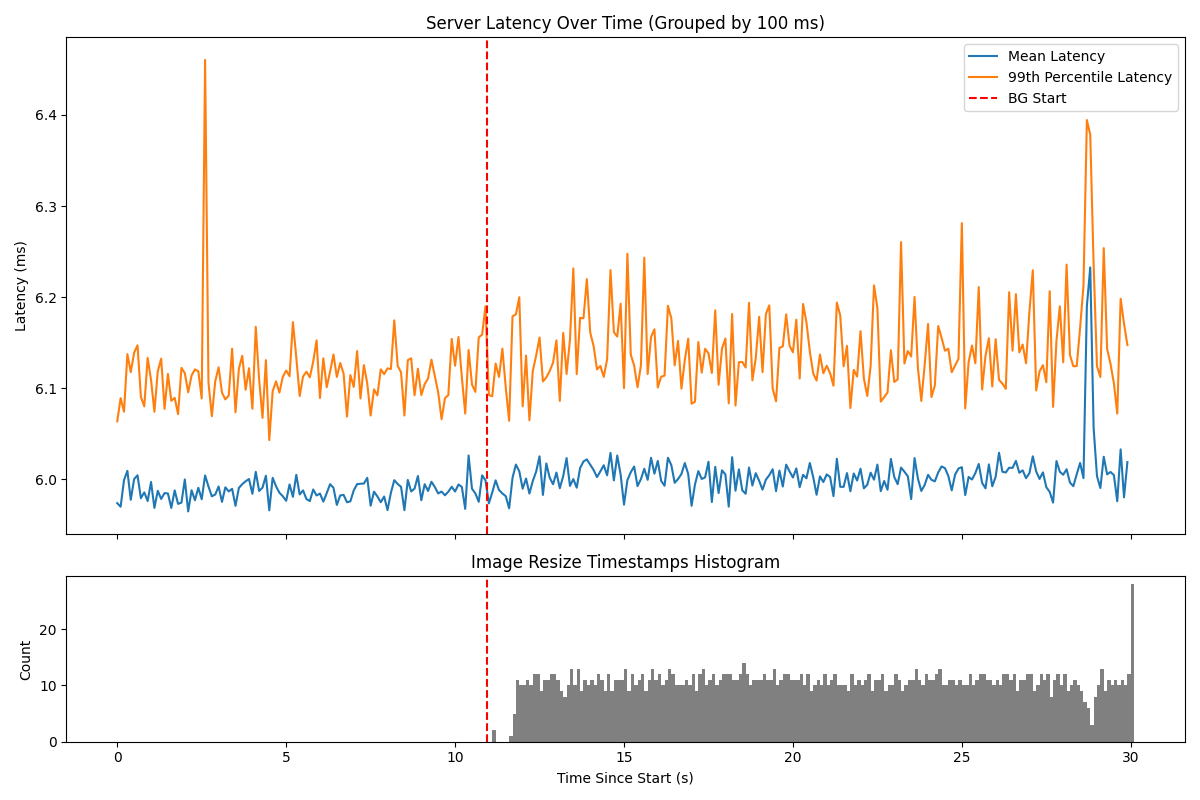
\includegraphics[width=\columnwidth]{graphs/srv-bg-rt-low.png}
        \caption{Low load}\label{fig:srv-bg-rt-low}
        \vspace{12pt}
    \end{subfigure}
    \hspace{\fill}
    \begin{subfigure}[t]{\columnwidth}
        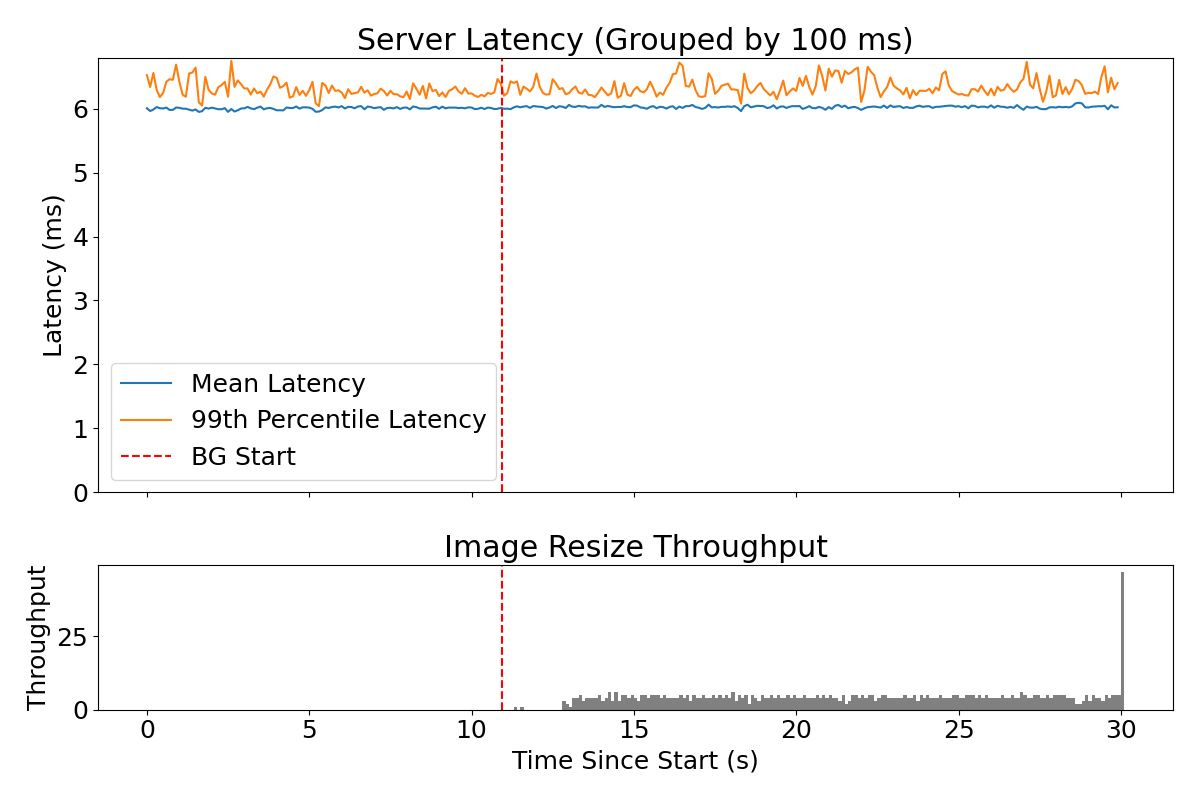
\includegraphics[width=\columnwidth]{graphs/srv-bg-rt-high.png}
        \caption{High load}\label{fig:srv-bg-rt-high}
    \end{subfigure}
    \vspace{4pt}
    \caption{Results of the same experiment as in \autoref{fig:srv-bg-unedited}
    and \autoref{fig:srv-bg-schedbe}, with LC running as a real time
    process}\label{fig:srv-bg-rt}
\end{figure}

\autoref{fig:srv-bg-rt} shows the result of running the same microbenchmark from
\autoref{fig:srv-bg-unedited}, but with the LC server in the \rtclass{}
scheduling class. We can see that \rtclass{} is isolated from \normalclass{}
well: in both load settings the tail and average latency stays stable at
$\sim$6.0ms.

However, running LC in \rtclass{} is an untenable way of isolating LC from BE
because of \rtclass{}'s intra-priority schedulers. \schedfifo{} uses
run-to-completion scheduling, which is known to have a failure mode of
head-of-line (HoL) blocking under varied request processing times, where
long-running requests monopolize the CPU while short requests wait in the queue.
\schedrr{} addresses this concern by running a round-robin scheduler that will
ensure Processor Sharing within priorities. However, \schedrr{} has no way way
of enforcing unequal splits, every process just gets the same scheduling quantum
and then gets put at the end of that priority's queue. Unequal splits is
precisely what weights are good at, and why they are used for LC services today.


\begin{figure}[t]
    \centering
    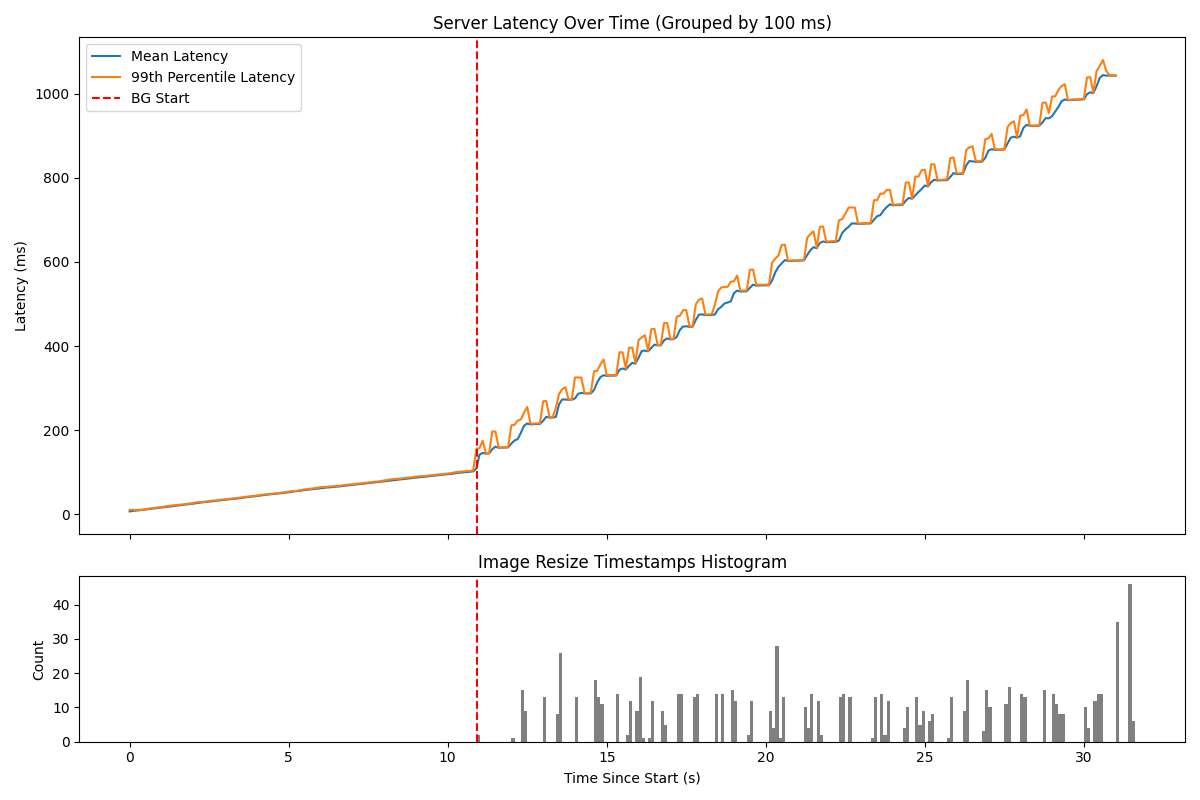
\includegraphics[width=\columnwidth]{graphs/overload-rt.png}
    \caption{LC in real time, throttling}\label{fig:overload-rt}
\end{figure}

In addition, under high utilization of real time processes, Linux does not park
the lower class processes or do something equivalent, but instead throttles the
\rtclass{} LC processes~\cite{lkml-deadline-srv}. We can see this happen when
we run the same microbenchmark experiment at a much higher baseline utilization
($\sim$ 100\%). The results are in \autoref{fig:overload-rt}. We see spikes
begin to appear after starting the BE task, as the \rtclass{} server gets
throttled in favor of running the BE tasks; we see parallel spikes in the BE's
throughput in the bottom graph. Notice also the increase of the slope of response
times after starting the background tasks.

We conclude that Linux's mechanism of scheduling classes can isolate workloads
effectively, but existing scheduling classes use algorithms that are not a good
fit for modern workloads, and throttle the higher class under high load.







